\chapter{Implementation}
In Computer Graphics, we generally synthesize 2d images from a given 3d scene description. This process is denoted as rendering. A usual computer graphics scene consist of a viewer's eye, modelled by a virtual camera, light sources and geometries placed in a world$\footnote{With the term world we are referring to a global coordinate system which is used in order to place all objects.}$, having some material properties$\footnote{Example material properties are: textures, surface colors, reflectance coefficients, refractive indices and so on.}$ assigned to them. In our implementation, scene geometries are modelled by triangular meshes for which each triangle is represented by a triplet of vertices. Each vertex has a position, a surface normal and a tangent vector associated with it. \\

The process of rendering basically involves a mapping of 3d scene objects to a 2d image plane and the computation of each image pixel's color according to the provided lighting, viewing and material information of the given scene. These pixel colors are computed in several stages in so called shader programs, directly running on a Graphic Processing Unit (GPU) hardware device. In order to interact with a GPU, for our implementations, we rely on the programming interface called OpenGL$\footnote{Official website:\texttt{http://www.opengl.org/}}$, a cross-language, multi-platform API. In OpenGL, there are two fundamental shading pipeline stages, the vertex- and the fragment shading stage, both applied sequentially. Vertex shaders apply all transformations to the mesh vertices and pass this data to the fragment shaders. Fragment shaders receive linearly interpolated vertex data of the respective particular triangle. They are responsible to compute the color of each fragment. \\

In this chapter we explain in detail a technique for rendering structural colors due to diffraction effects on natural gratings, based on the model we have derived in the previous chapter $\ref{chap:derivations}$, summarized in section $\ref{sec:spectralrendering}$. For this purpose we implemented a reference framework which is based on a class project for a course in \emph{Computer Graphics} held by Prof. M. Zwicker which I attended in autumn 2012$\footnote{The code of underlying reference framework is written in Java and uses JOGL and GLSL$\footnotemark$ in order to communicate with the GPU and can be found at \texttt{https://ilias.unibe.ch/}}$. \\
$\footnotetext{JOGL is a Java binding for OpenGL (official website \texttt{http://jogamp.org/jogl/www/}) and GLSL is OpenGL's high-level shading language. Further information can be found on wikipedia: \texttt{http://de.wikipedia.org/wiki/OpenGL\textunderscore Shading\textunderscore Language}}$

For rendering process, our implementation needs the following input data$\footnote{All data is provided by the Laboratory of Artificial and Natural Evolution in Geneva. See their website:\texttt{www.lanevol.org}}$:
\begin{itemize}
  \item The raw structure patch for a snake skin$\footnote{We are using height field data for Elaphe and Xenopeltis snakes as shown in figure $\ref{fig:snakespecies}$}$ represented as discrete height fields acquired using AFM and stored as grayscale images.
  \item Real measured snake geometry represented as a triangle mesh.
  \item A vector field indicating local orientation for the patch over the triangular mesh.
  \item Optional texture data representing pigmentation for the snake skin.
\end{itemize}

The first processing stage of our implementation is to compute the Fourier Terms of the provided height fields as described in section $\ref{sec:taylorapproximation}$. For this preprocessing purpose we use Matlab relying on its internal, numerically fast, libraries for computing Fourier Transformations$\footnote{Actually we use Matlab's inverse 2d Fast Fourier Transformation (FFT) implementation applied on different powers of equation $\ref{eq:px}$. Further information can be read up in section $\ref{sec:precompmatlabfourierimages}$}$. The next stage is to read these precomputed Fourier Terms into our Java renderer. This program also builds our manually defined rendering scene. The last processing stage of our implementation is rendering of the iridescent color patterns due to light diffracted on snake skins. We implemented our diffraction model from chapter $\ref{chap:derivations}$ as OpenGL shaders. Notice that all the necessary computations in order to simulate the effect of diffraction are performed within a fragment shader. This implies that we are modelling pixel-wise the effect of diffraction and hence the overall rendering quality and runtime complexity depends on rendered window's resolution. \\

In the following sections of this chapter we are going to explain all render processing stages in detail. First, we discuss how our precomputation process, using Matlab, actually works. Then, we introduce our Java Framework. It is followed by the main section of this chapter, the explanation of how our OpenGL shaders are implemented. The last section discusses an optimization of our fragment shader such that it will have an interactive runtime.

\section{Precomputations in Matlab}
\label{sec:precompmatlabfourierimages}
Our first task is to precompute the two dimensional discrete Fourier Transformations for a given input height field, representing a natural grating. For that purpose we have written a small Matlab $\footnote{Matlab is a interpreted scripting language which offers a huge collection of mathematical and numerically fast and stable algorithms.}$ script conceptualized in algorithm $\ref{alg:matlabprecomp}$. Our Matlab script reads a given grayscale image, which is representing a nano-scaled height field, and computes its two dimensional DFT (2dDFT) by using Matlab's internal Fast Fourier Transformation (FFT) function, denoted by $ifft2$$\footnote{Remember, even we are talking about Fourier Transformations, in our actual computation, we have to compute the inverse Fourier Transformation. See paragraph $\ref{sec:electricalengeneeringftconvention}$ for further information. Furthermore our height fields are two dimensional and thus we have to compute a 2d inverse Fourier Transformation.}$. Keep in mind that taking the Fourier transformation of an arbitrary function will result in a complex valued output which implies that we will get a complex value for each frequency pairs in the discretized 2d frequency space. Therefore, for each input image we get as many output images, representing the 2dDFT, as the minimal number of taylor terms required for a well-enough approximation. In order to store our output images, we use two separate color channels to store the real and imaginary parts of the DFT coefficients. Some example visualizations for the Fourier Transformation are shown in figure $\ref{fig:matlabBlazeFourierImages}$. We store these intermediate results as binary files to support floating point precision for the run-time computations. \\

In our script, every DFT coefficient is normalized by its corresponding DFT range extrema$\footnote{We are talking about the i2dFFT of our height fields when raised to the power of n. This is an N by N matrix (assuming the discrete height field was an N by N image), for which each component is a complex number. Hence, there is a real extrema pair as well as a imaginary extrema pair of max and min.}$ to the range $\left[0,1\right]$ and the range extrema are stored separately for each DFT term. The normalization is computed the following way: 

\begin{align}
  f:\left[x_{min},x_{max}\right]\to \left[0,1\right] \nonumber\\
  x \mapsto f(x) = \frac{x-x_{min}}{x_{max}-x_{min}}
\label{eq:dfttermnormalization}
\end{align}

Where $x_{min}$ and $x_{max}$ denote the extreme values of a DFT term. Later, during the shading process of our implementation, we have to apply the inverse mapping. This is a non-linear interpolation which is required in order to rescale all frequency values in the DFT terms. 

\begin{algorithm}[H]
\caption{Precomputation: Pseudo code to generate Fourier terms}
\textbf{INPUT} \ $heightfieldImg, \ maxH, \ dH, \ termCnt$ \\
\textbf{OUTPUT} \ $DFT \ terms \ stored \ in \ Files$
\begin{lstlisting}
% maxH:    A floating-point number specifying 
%          the value of maximum height of the 
%          height-field in MICRONS, where the 
%          minimum-height is zero. 
%         
% dH:      A floating-point number specifying 
%          the resolution (pixel-size) of the 
%          'discrete' height-field in MICRONS. 
%          It must be less than 0.1 MICRONS 
%          to ensure proper response for 
%          visible-range of light spectrum.
%
% termCnt: An integer specifying the number of 
%          Taylor series terms to use.

function ComputeFFTImages(heightfieldImg, maxH, dh, termCnt)
dH = dh*1E-6;
% load patch into heightfieldImg
patchImg = heightfieldImg.*maxH;
% rotate patchImg by 90 degrees
for t = 0 : termCnt
  patchFFT = power(1j*patchImg, t);
  fftTerm{t+1} = fftshift(ifft2(patchFFT));
  
  % rescale terms as
  imOut(:,:,1)  = real(fftTerm{t+1});
  imOut(:,:,2)  = imag(fftTerm{t+1});
  imOut(:,:,3)  = 0.5;
  
  % rotate imOut by -90 degrees
  % find real and imaginary extrema of 
  % i.e. the max. and min. for both real and imaginary parts
  % rescale real and imaginary parts using equation 4.1
  % write imOut 
  % write extremas into files.
end
\end{lstlisting}
\label{alg:matlabprecomp}
\end{algorithm}

They key idea of algorithm $\ref{alg:matlabprecomp}$ is to compute iteratively the Fourier Transformation for different powers of the provided height field. These DFT values are scaled by according to their extrema values. Another note about the command fftshift: It rearranges the output of the ifft2 by moving the zero frequency component to the centre of the image. This simplifies the computation of DFT terms lookup coordinates during rendering.


\label{sec:precompmatlabfft}
\begin{figure}[H]
  \newcounter{foo}
  \centering
  \subfigure[Heightfield of a Blazed grating]{
    
\includegraphics[scale=0.32]{implementation/hf/blaze/blazeBig.png}
    \label{fig:matlabBlazePatch}
  }
~
  \subfigure[Plot of extreme values for different powers $N$ for the Blazed grating]{
    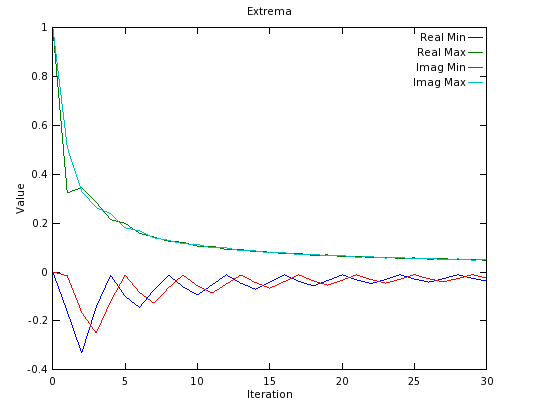
\includegraphics[scale=0.5]{implementation/extrema.png}
    \label{fig:extremaBlaze}  
  }
  
  \caption[Blazed Grating with its Extrema]{Illustration of a Blazed grating and a plot of how the extrema of its DFT terms.}
  \label{blazedgratingextrema}
\end{figure}


\begin{figure}[H]
  \begin{table}[H]
    \begin{center}
      \begin{tabular}{@{}lllcl@{}} 
      \subfigure[ImRe0]{
        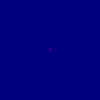
\includegraphics[scale=0.65]{implementation/hf/blaze/AmpReIm0.png}
        \label{fig:blazeftimre0}
      }&
      \subfigure[ImRe10]{
        
\includegraphics[scale=0.65]{implementation/hf/blaze/AmpReIm10.png}
        \label{fig:blazeftimre10}
      }&   
      \multirow{10}{15em}{
          \subfigure[ImRe20]{
            
\includegraphics[scale=2.23]{implementation/hf/blaze/AmpReIm20.png}
            \label{fig:blazeftimre20}
          }
      }\\
      \subfigure[Re0]{
        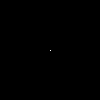
\includegraphics[scale=0.65]{implementation/hf/blaze/re0.png}
        \label{fig:blazeftre0}
      }& 
      \subfigure[Re10]{
        
\includegraphics[scale=0.65]{implementation/hf/blaze/re10.png}
        \label{fig:blazeftre10}
      }&\\ 
      \subfigure[Im0]{
        
\includegraphics[scale=0.48]{implementation/hf/blaze/im0.png}
        \label{fig:blazeftim0}
      }& 
      \subfigure[Im10]{
        
\includegraphics[scale=0.65]{implementation/hf/blaze/im10.png}
        \label{fig:blazeftim10}
      }&\\ 
      \end{tabular}
    \end{center}
  \end{table} 
  \caption[DFT Terms for a Blazed Grating]{A visualization of the DFT terms for a height field representing a Blazed grating.}
  \label{fig:matlabBlazeFourierImages}
\end{figure}

In figure $\ref{fig:matlabBlazeFourierImages}$ we see examples for a visualization of Fourier transformations generated by our Matlab script with a Blazed grating$\footnote{A Blazed grating is a height field consisting of ramps, periodically aligned on a given surface.}$ as an input height field image, shown in figure $\ref{fig:matlabBlazePatch}$. Figure $\ref{fig:extremaBlaze}$ shows plots of the extreme values of DFT terms for different powers $N$ of the height field. We recognize that, the higher the power of the grating becomes, the closer the extreme values of the corresponding DFT terms get. The figure line from figure $\ref{fig:matlabBlazeFourierImages}$(a) until figure $\ref{fig:matlabBlazeFourierImages}$(b) show us exemplarily, visualizations of DFT terms for different powers $N$ of our grating's height field. Remember that DFT terms are complex valued matrices of dimensions same as that for their corresponding height field. In this visualization, all real part values are stored in the red- and the imaginary parts in the green color channel of image. The figure line from figure $\ref{fig:matlabBlazeFourierImages}$(d) till figure  $\ref{fig:matlabBlazeFourierImages}$(e) show us the real part images from the figures in the line above. Similarly for the figure line from figure  $\ref{fig:matlabBlazeFourierImages}$(f) until figure  $\ref{fig:matlabBlazeFourierImages}$(g) showing the corresponding imaginary parts of the DFT terms. Figure $\ref{fig:matlabBlazeFourierImages}$(c) is a visualization of a scaled DFT term of a Blazed grating. In this visualization we only see color contribution along the x-axis. Reason for this is, that, since a blazed grating only varies along the x-axis, also its corresponding 2d DFT image will vary only at the x-axis. 

\section{Java Renderer}
This section explains the architecture of the rendering program which I implemented$\footnote{This program is based on the code of a java real-time renderer, developed as a student project in the \emph{Computer Graphics} class, held by M. Zwicker in autumn 2012. A basic implementation of a rendering engine called \emph{jrtr} was provided in this class.}$ and used for this project. The architecture of the program is divided into two parts: a rendering engine, the so called jrtr (java real time renderer) and an application program. Figure $\ref{fig:rendererArchitecture}$ outlines the architecture of the renderer. 

\begin{figure}[H]
  \centering
  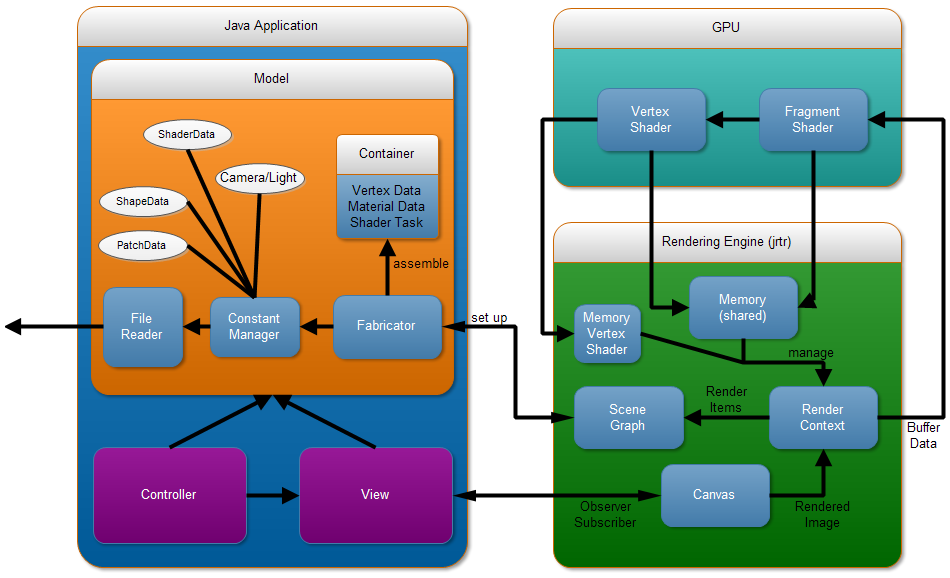
\includegraphics[scale=0.63]{implementation/renderingarch.png}
  \caption[Architecture of Renderer]{Schematical architecture of our Java renderer. An arrow which is pointing from A to B indicates that A requests some data from B.}
  \label{fig:rendererArchitecture}
\end{figure}

The application program relies on the MVC (Model-View-Controller) architecture pattern. The View represents a canvas in which the rendered images are shown. The Controller implements the event listening functionalities for interactive rendering within the canvas. The Model of our application program consists of a Fabricator, a file reader and a constants manager. The main purpose of a Fabricator is to set up a rendering scene by accessing a constant manager containing many predefined scene constants. A scene consists of a camera, a light source, a view frustum, shapes and their associated material constants. Such materials include a shape texture, precomputed DFT terms$\footnote{See section \ref{sec:precompmatlabfourierimages} for further information.}$ for a given height field$\footnote{and other height field constants such as the maximal height of its bumps or its pixel real-world width correspondance.}$ as visualized in figure $\ref{fig:matlabBlazeFourierImages}$. A shapes is a geometrical object defined by a triangular mesh as shown in figure $\ref{fig:wireframemesh}$. 

\begin{figure}[H]
  \centering
  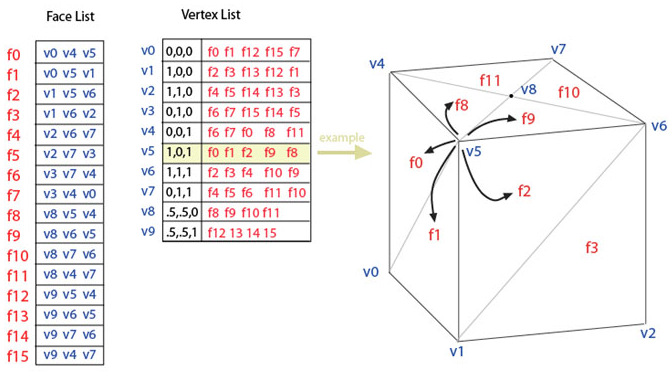
\includegraphics[scale=0.7]{implementation/wireframemesh.png}
  \caption[Triangular Mesh]{Representation$\footnotemark$ of a triangular mesh represents an object as a set of triangles and a set of vertices.}
  \label{fig:wireframemesh}
\end{figure}
\footnotetext{Modified image which originally has been taken from \texttt{http://en.wikipedia.org/wiki/Polygon\textunderscore mesh}}

Such a mesh is represented as a data structure consisting of a list of vertices, each stored as a triplet of $x$, $y$, $z$ positions and triangles, each defined by a triple of vertex-indices. Besides its position, a vertex can have further data assigned to, like a surface color, normals and texture coordinates. The whole scene is encapsulated in a scene graph data-structures, defined and managed within the rendering engine. A scene graph contains all scene geometries and their transformations in a tree like structured hierarchy. \\

All required configuration, in order to communicate with the GPU through OpenGL, is set in the jrtr rendering engine. Furthermore, the whole resource-management for various types of low-level buffers which are used within the rendering pipeline by our GLSL shaders is cloned by the renderer context object. More precisely, this means allocating memory for the buffers, assigning them to scene data and flushing them, when not used anymore. The whole shading process is performed in the GPU, stage-wise: The first stage is the vertex shader (see section $\ref{sec:vertexshader}$) followed by the fragment shader (see section $\ref{sec:fragmentshader}$). The jrtr framework also offers the possibility to assign user-defined shaders written in GLSL.

\section{GLSL Diffraction Shader}
\subsection{Vertex Shader}
\label{sec:vertexshader}
In our implementation we want to simulate the structural colors that a viewer sees when light is diffracted from a grating, e.g. the skin of a snake. For this purpose, we reproduce a 2d image of a given 3d scene as seen from the perspective of a viewer for given lightning conditions. The color computation of an image is performed in the GPU shaders of the rendering pipeline. In OpenGL, there are two basic shading stages performed to render an image where the vertex shader is the first shading stage in the rendering pipeline. \\

As an input, a vertex shader, as illustrated in figure $\ref{fig:vertexshaderpipe}$, receives one vertex of a mesh at a time and all the other vertex data associated with it such as a vertex normal. It can only access this data and has no information about the neighborhood of a vertex or the topology of its corresponding shape. Since vertex positions of a shape are defined in a local coordinate system$\footnote{Defining the positions of a shape in a local coordinate system simplifies its modelling process and allows us to apply transformations to a shape.}$ and we want to render an image for the perspective of a viewer, we have to perspectively project(transform) the locally defined positions to a viewer's 2D space. Therefore, the main purpose$\footnote{Furthermore, texture coordinates used for texture-lookup within the fragment shader and per vertex lightning can be computed.}$ of a vertex shader is to transform the position of vertices from a local 3D space to a viewer's 2D image space. Notice that a vertex shader can manipulate the position of a vertex, but cannot generate additional mesh vertices. Therefore, the output of any vertex shader is a transformed vertex position. Keep in mind that all vertex shader outputs will be used within the fragment shader. For an example, please have a look at our fragment shader $\ref{sec:fragmentshader}$. \\

\begin{figure}[H]
  \centering
  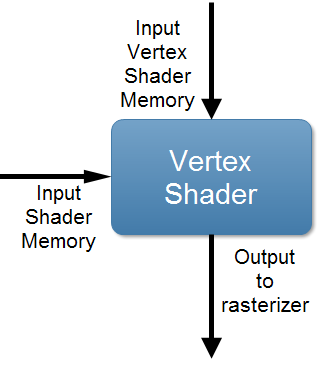
\includegraphics[scale=0.5]{implementation/vertexshader.png}
  \caption[Vertex Shader]{Illustration of vertex shader in OpenGL's rendering pipeline.}
  \label{fig:vertexshaderpipe}
\end{figure}

In the following let us consider the whole transformation, as applied in a vertex shader, in depth. Let $p_{local}$ denote the position of a shape vertex, defined in a local coordinate system. Then the transformation from $p_{local}$
into the perspective projected position as seen by a observer $p_{projective}$ looks like the following:

\begin{equation}
  p_{projective} = P \cdot C^{-1} \cdot M \cdot p_{local}
  \label{eq:vertextransformation}
\end{equation}

where $P$, $C^{-1}$ and $M$ are transformation matrices$\footnote{These transformation matrices are linear transformations expressed in homogenous coordinates.}$, defined the following way:

\begin{description}
\item[Model matrix $M$:] Each vertex position of a shape is initially defined in a local coordinate system. To make it feasible to place and transform shapes in a scene, a reference coordinate system, the so called world space, has to be introduced. Hence, for every shape a matrix $M$ is associated, defining the transformation from its local coordinate system into the world space. 
\item[Camera matrix $C$:] A camera models how the eye of a viewer sees an object defined in a world space as shown in figure $\ref{fig:cameracoordinatesystem}$. $C$ denotes a transformation from coordinates defined in the camera space into the world space. For calculating the transformation matrix $C$, a viewer's eye position and viewing direction, each defined in world space, are required. In order to transform a position from world space to camera space, we have to use the inverse of $C$, denoted by $C^{-1}$. 
\item[Frustum $P$:] The Matrix P defines a perspective projection onto the image plane, i.e. for any given position in camera space, $P$ determines the corresponding 2d image coordinate. Perspective projections project along rays that converge at the center of projection.
\end{description}

Since we are interested in modelling how a viewer sees structural colors on a given scene shape as shown in figure $\ref{fig:cameracoordinatesystem}$, modelling a viewer's eye by formulating the corresponding camera matrix $C$, is an important component of the whole transformation series applied in the vertex shader. Hence, we next will have a closer look in how a camera matrix $C$ actually can be computed. 

\begin{figure}[H]
  \centering
  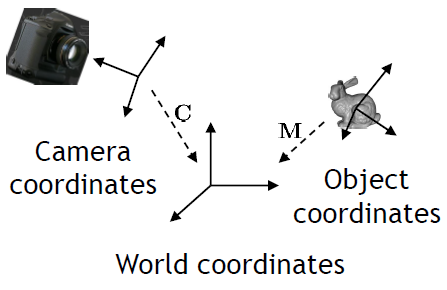
\includegraphics[scale=0.7]{implementation/cameracoodsyst.png}
  \caption[Camera Coordinate System]{Illustration$\footnotemark$ of the Camera coordinate system where its origin defines the center of projection of the camera.}
  \label{fig:cameracoordinatesystem}
\end{figure}
\footnotetext{This image has been taken from the lecture slides of computer graphics class 2012 which can be found on Ilias.}

The camera matrix $C$ is constructed from its center of projection $e$, the position $d$ where the cameras looks at and a direction vector $up$, defining what is the direction in camera space pointing upwards. These components, $e$, $d$ and $up$, are defined in world coordinates. Figure $\ref{fig:cameramatrix}$ illustrates the geometrical setup required in order to construct $C$.

\begin{figure}[H]
  \centering
  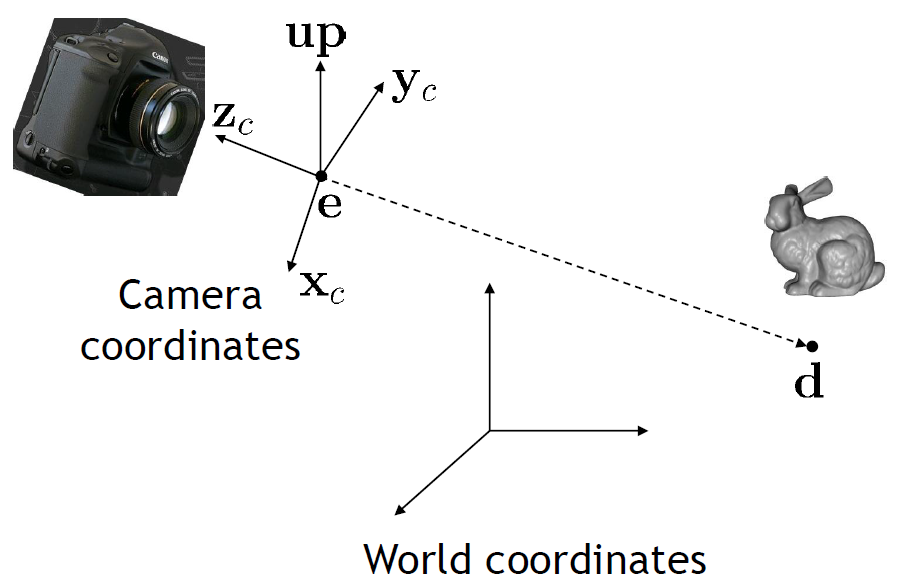
\includegraphics[scale=0.35]{implementation/cameramatrix.png}
  \caption[Camera Matrix]{Illustration$\footnotemark$ of involved components in order to construct the camera matrix $C$. The eye-vector $e$ denotes the position of the camera in space, $d$ is the position the camera looks at, and $up$ denotes the cameras height. The camera space is spanned by the helper vectors $x_c$, $y_c$ and $z_c$. Notice that objects we look at are in front of us, and thus have negative $z$ values}
  \label{fig:cameramatrix}
\end{figure}
\footnotetext{This image has been taken from the lecture slides of computer graphics class 2012 which can be found on ILIAS.}

The mathematical representation of these vectors, $x_c$, $y_c$ and $z_c$, spanning the camera space, introduced in figure $\ref{fig:cameramatrix}$, looks like the the following: 

\begin{align}
  &z_c = \frac{e-d}{||e-d||} \nonumber \\
  &x_c = \frac{up \times z_c}{||up \times z_c||} \nonumber \\
  &y_c = z_c \times x_c
  \label{eq:cameraspacespanningvectors}
\end{align}

As we can see, $x_c$, $y_c$ and $z_c$ are independent unit vectors. Therefore, they span a 3d space, the so called camera matrix. In order to express a coordinate in camera space, we have to project it onto these unit vectors. Using a homogenous coordinates representation, this projection onto these unit vectors can be formulated by the transformation matrix $C$:

\begin{equation}
  C = \begin{bmatrix} x_c & y_c & z_c & e \\ 0 & 0 & 0 & 1 \end{bmatrix}
  \label{eq:cameramatrixeq}
\end{equation}

In our vertex shader, besides transforming the vertex positions as described in equation $\ref{eq:vertextransformation}$, for every vertex, we also compute the direction vectors $\omega_i$ and $\omega_r$ described like in figure $\ref{fig:geometricsetup}$. Those direction vectors are transformed onto the tangent space, a local coordinate system spanned by a vertex's normal, tangent and binormal vectors. For further information and more insight about the the \emph{tangent space}, please have a look at the appendix in the section $\ref{sec:tangentspace}$. The algorithmic idea of our vertex shader, stating all its computational steps, is conceptualized in algorithm $\ref{alg:vertexshader}$.

\begin{algorithm}[H]
\caption{Vertex diffraction shader pseudo code}
\begin{table}[H]
  \begin{tabular}{@{}lll@{}}
    \textbf{Input:} & \emph{Mesh} with vertex \emph{normals} and \emph{tangents}  \\
    & Space transformations $\{M, C^{-1}, P\}$  \\
    & Light direction \emph{lightDirection}  \\
    \textbf{Output:} & Incident light and viewer direction $\omega_i,\ \omega_r$ \\
    & Transformed position $p_{per}$ \\
  \end{tabular} 
\end{table}
\textbf{Procedures:} $normalize()$, $span()$, $projectVectorOnTo()$  \\
\setlength{\fboxrule}{0pt} 
\begin{boxedminipage}{1.0\textwidth}
  \begin{algorithmic}[1]
      \ForAll{$VertexPosition \thinspace position \in Mesh$}
        \State $ vec3 \ N = normalize(M * vec4(normal,0.0).xyz)$
        \State $ vec3 \ T = normalize(M * vec4(tangent,0.0).xyz)$
        \State $ vec3 \ B = normalize(cross(N, T))$
        \State $ TangentSpace = span(N, T, B)$
        \State $ viewerDir = ((cop_{w}-position)).xyz$
        \State $ lightDir = normalize(lightDirection)$
        \State $ \omega_i = projectVectorOnTo(lightDir, TangentSpace)$
        \State $ \omega_r = projectVectorOnTo(viewerDir, TangentSpace)$
        \State $normalize(\omega_i); \ normalize(\omega_r)$
        \State $p_{per} = P \cdot C^{-1} \cdot M \cdot p_{obj}$
      \EndFor
  \end{algorithmic}
  \end{boxedminipage}
  \vskip1.5pt
\label{alg:vertexshader}
\end{algorithm}

As input, our vertex shader algorithm $\ref{alg:vertexshader}$ takes a mesh with of a given scene shape. Each of this vertex should have a normal and a tangent assigned to. Furthermore, the direction of the scene light is required. For our implementation we always used directional light sources. An example of an directional light source is given in figure $\ref{fig:dirlightsource}$. 

\begin{figure}[H]
  \centering
  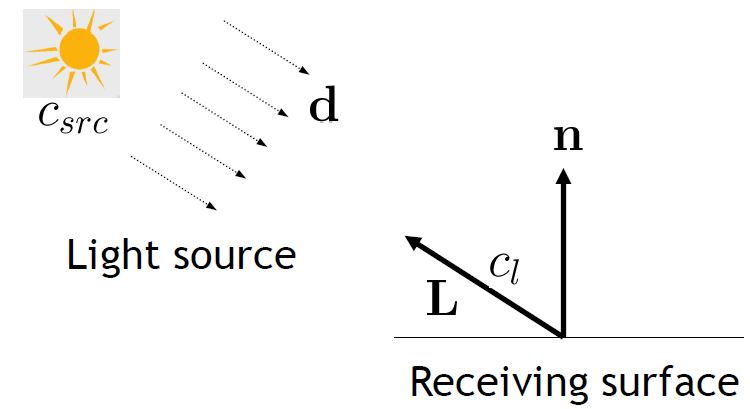
\includegraphics[scale=0.45]{implementation/dirlightsource.png}
  \caption[Rays of a Directional Light]{Illustration$\footnotemark$ of our light source setup. For a directional light source, all light rays are in parallel.}
  \label{fig:dirlightsource}
\end{figure}
\footnotetext{This image has been taken from the lecture slides of computer graphics class 2012 which can be found on ILIAS.}

Last, in order to transform the positions of our mesh as described in equation $\ref{eq:vertextransformation}$, we also have to pass these transformation matrices$\footnote{When speaking about transformation matrices, we are refering to the model, camera and frustum matrices.}$. For simplification purposes, we introduced the following helper procedures used in the vertex shading algorithm:

\begin{description}
  \item[normalize():] Computes the normalized version of a given input vector.
  \item[span():] Assembles a matrix from a given set of vectors. This matrix spans a vector space.
  \item[projectVectorOnTo():] Takes two arguments, a vector and the matrix. The first argument is projected onto each column of a given matrix. It returns a vector in the space spanned by the columns of the given argument matrix.
\end{description}

The output of our vertex shader includes the transformed vertex position, the incident light $\omega_i$ and viewing direction $\omega_r$ both transformed into the local tangent space at that vertex. The output of the vertex shader is used as the input of the fragment shader, as discussed in the next section.

\subsection{Fragment Shader}
\label{sec:fragmentshader}
In the previous section we gave an introduction to the first shading stage of the OpenGL rendering pipeline by explaining the basics of a vertex shader. Furthermore, we conceptually discussed the idea behind our vertex shading algorithm formulated in algorithm $\ref{alg:vertexshader}$. Summarized, the main purpose of our vertex shader is to compute the light- and viewing-direction vectors $\omega_i$ and $\omega_r$ defined like in figure $\ref{fig:geometricsetup}$. \\

After the vertex-shading stage, the next stage in the OpenGL rendering pipeline is the \emph{rasterization} of mesh triangles. As an input, a rasterizer takes a triplet of mesh-triangle spanning vertices, each previously processed by a vertex shader. For each pixel lying inside the current mesh triangle, a rasterizer computes its corresponding position in the triangle. According to its computed position, a pixel also gets interpolated values of the vertex attributes assigned to its mesh triangle. The set of interpolated vertex attributes together with the computed position of a pixel is denoted as a fragment. Figure $\ref{fig:trianglerasterization}$ conceptualizes the idea of processed set of fragment computed by a rasterizer.

\begin{figure}[H]
  \centering
  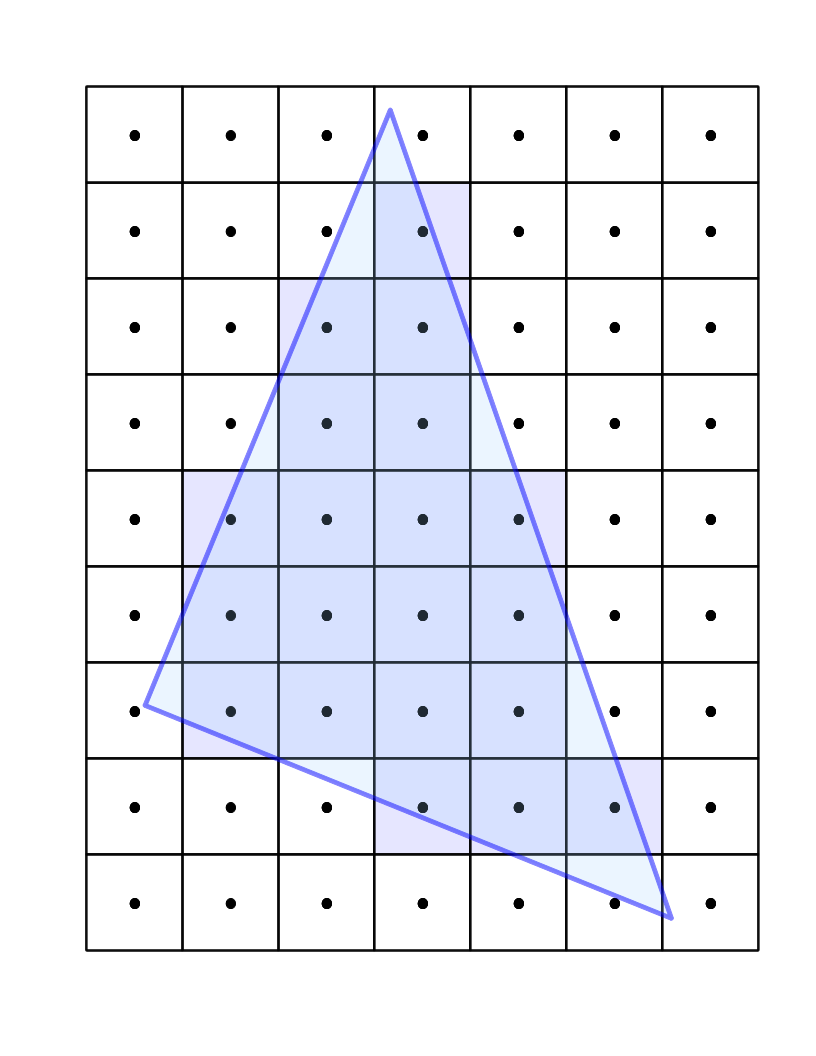
\includegraphics[scale=0.25]{implementation/rasterizedtriangle.png}
  \caption[Triangle Rasterization]{Illustration$\footnotemark$ of fragments covered by a mesh triangle computed by the OpengGL rasterizer.}
  \label{fig:trianglerasterization}
\end{figure}
\footnotetext{This image was taken from \texttt{http://en.wikibooks.org/wiki/GLSL\textunderscore Programming/Rasterization}}

A fragment shader as shown in figure $\ref{fig:fragmentshaderpipe}$, is the OpenGL pipeline stage subsequent to the rasterization stage. As input value, a fragment shader takes at least a fragment computed by the rasterizer. It is also possible to assign custom, non-interpolated values to a fragment shader. For each fragment in the fragment shading stage, a color value is computed. Furthermore, a fragment shader computes a depth value for each of its fragments, determining their visibility. Since all existing scene vertices were perspectively projected onto the 2d image plane, the rasterizer could have produced several fragments having assigned the same pixel position. Therefore, among all fragments with the same pixel position, the output pixel color for opaque fragments is equal to the color of the fragment, which is closest to the viewer.

\begin{figure}[H]
  \centering
  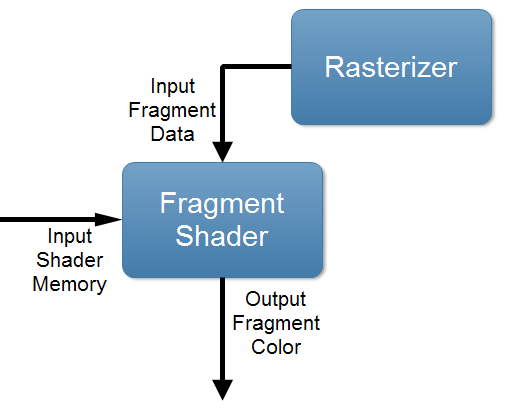
\includegraphics[scale=0.5]{implementation/fragmentshader.png}
  \caption[Fragment Shader]{Illustration of fragment shader in OpenGL's rendering pipeline.}
  \label{fig:fragmentshaderpipe}
\end{figure}

\label{sec:flssshader}
\label{sec:inputlists}
In this section we explain how to render structural colors resulting due to light diffracted on a natural grating, based on the model described in section $\ref{sec:spectralrendering}$ in equation $\ref{eq:finalexpression}$. The color values of the produced structural colors, resulting from our model, are computed by our fragment shader (later denoted as $\textbf{FLSS}$) which expects being provided by the following input:

\begin{itemize}
  \item Precompute DFT terms of the provided height field as explain in section $\ref{sec:precompmatlabfourierimages}$.
  \item The processed output, produced during the vertex shading stage (see section $\ref{sec:vertexshader}$), which is, the light- and viewing-direction vectors $\omega_i$ and $\omega_r$.
  \item Fragments produced during the rasterization stage using the output of our vertex shader.
\end{itemize}

Apart from these basic input values, the following set of shading constants are initialized:

\begin{itemize}
  \item The number of iterations used for the taylor series approximation, determining the the approximation accuracy.
  \item The wavelength spectrum $\Lambda = [\lambda_{min}, \lambda_{max}]$ with a certain discretizing level $\lambda_{step}$.
  \item The color weights of the $CIE_{XYZ}$ color matching functions.
  \item The height field image resolution and its sampling rate $dH$$\footnote{In other words dH indicates the pixel size in the height field image, i.e. what is the width and height of one pixel.}$.
\end{itemize}

By using all these inputs, our fragment shader performs a numerical integration over the given wavelength spectrum $\Lambda$ for our final derived expression, stated in equation $\ref{eq:finalexpression}$. For this integration we use the trapezoidal-rule with uniform discretization of the wavelength spectrum at $\lambda_{step}=5nm$ step sizes. This implies we are compressing sampled frequencies to the region near the origin due to the fact we are dividing the $(u,v)$ by the wavelength $\lambda$ and this implies that the $(u,v)$ space is sampled non-linearly. \\

In section $\ref{sec:gaussianwindow}$ we have seen that we have to multiply our DFT terms by a Gaussian Window in order to approximate the DTFT which our model is based on. This windowing approach is performed for each discrete $\lambda$ value using a window large enough to span $4\sigma_f$ in both dimensions. Our DFT terms are computed from height fields that span at least 65$\mu m^2$ and are sampled at a resolution of at least 0.1$\mu m$ . 
This ensures that the spectral response encompasses all the wavelengths in the visible spectrum. \\

\label{sec:proceduresdescripton}
Next, we will discuss the actual fragment shading algorithm, listed in algorithm $\ref{alg:fragmentshaderall}$. Note, that our fragment shading algorithm uses some helper procedures. One of the two most fundamental helper procedures is the $\textbf{getlookupCoords}$ which computes the lookup coordinates in the DFT terms for a given (u,v) defined like in equation $\ref{eq:uvw}$ and a wavelength $\lambda$. The actual computation of these coordinates is described in section $\ref{sec:texturelookupcoords}$. Notice that the routine $\textbf{getLocalLookUp}$ computes local lookup coordinates used during the gaussian window approximation explained in section $\ref{sec:gaussianwindow}$. The routine $\textbf{distVecFromOriginTo}$ computes a direction vector pointing from the current position of a fragment in texture space to one of its n-neighborhood neighbors (also living in the texture space). This direction vector is used for our Gaussian windowing approach where $n$ denotes the width of our window. 

\begin{algorithm}[H]
  \caption{Fragment diffraction shader pseudo code}
  \begin{table}[H]
    \begin{tabular}{@{}lll@{}}
      \textbf{Input:} & Normalized precomputed DFT terms along with extremas \\
      & A fragment from the rasterizer \\
      & Color matching functions \\
      & $\omega_i$ and $\omega_r$  \\
      & Frequency variance $\sigma_f$ \\
      \textbf{Output:} & Structural Color of a pixel \\
      \textbf{Procedures$\footnotemark$:} & $\emph{getColorWeights}$: get colormatching value for wavelength $\lambda$(see section \ref{sec:colorspace})\\
      & $\emph{getlookupCoords}$: get lookup coordinate(Eq.\ref{eq:ublookup}) by viewing-\& light direction \\
      & $\emph{distVecFromOriginTo}$: get direction vector from origin to a given position \\
      & $\emph{getLocalLookUp}$: get lookup coordinate(Eq.\ref{eq:gaussianwindowlook}) of DFT windowing values \\
      & $\emph{rescaledFourierValueAt}$: rescales DFT terms according to equation \ref{eq:dfttermnormalization}\\
      & $\emph{gaussWeightOf}$: computes gaussian window according to equation \ref{eq:gaussweight} \\
      & $\emph{dot}$: computes the dot-product of two given vectors \\
      & $\emph{gammaCorrect}$: apply gamma correction on RGB vector(see section \ref{subsec:colortransformations}) \\ 
      & $\emph{C}$: gain factor (see Eq. \ref{eq:cfact}) \\  
      & $\emph{shadowF}$: shadowing function (see the appendix of Stam's paper$\cite{diffstam}$) \\   
    \end{tabular} 
  \end{table}
  
  \setlength{\fboxrule}{0pt} 
  \begin{boxedminipage}{1.0\textwidth}
  \begin{algorithmic}[1]
    \ForAll{$Pixel \thinspace p \in Fragment$}
      \State \init $BRDF_{XYZ}, BRDF_{RGB}$ \myto $vec4(0.0)$
      \State $(u,v,w) = -\omega_i - \omega_r$
      \For{$(\lambda = \lambda_{min};\thinspace \lambda \leq \lambda_{max};\thinspace \lambda = \lambda + \lambda_{step})$}
        \State $xyzWeights = getColorWeights(\lambda)$
        \State $lookupCoord = getlookupCoords(u, v, \lambda)$
        \State \init $P$ \myto $vec2(0.0)$
        \State $k = \frac{2\pi}{\lambda}$
        \For{$(n = 0$ \myto $T)$}
          \State $taylorScaleF = \frac{(kw)^n}{n!}$
          \State \init $F_{fft}$  \myto $vec2(0.0)$
          \State $anchorX = int(floor(center.x + lookupCoord.x * fftImWidth)$
          \State $anchorY = int(floor(center.y + lookupCoord.y * fftImHeight)$
          \For{$(i=(anchorX-winW)$ \myto $(anchorX + winW))$}
            \For{$(j=(anchorY - winW)$ \myto $(anchorY + winW))$}
              \State $dist = distVecFromOriginTo(i,j)$
              \State $pos = getLocalLookUp(i,j,n)$
              \State $fftVal = rescaledFourierValueAt(pos)$
              \State $fftVal \asteq gaussWeightOf(dist, \sigma_f)$
              \State $F_{fft} \pluseq fftVal$
            \EndFor
          \EndFor
          \State $P \pluseq taylorScaleF*F_{fft}$
        \EndFor
        \State $xyzPixelColor \pluseq dot(vec3(\left|P\right|^2), xyzWeights)$
      \EndFor
      \State $BRDF_{XYZ} = xyzPixelColor*C(\omega_i, \omega_r)*shadowF(\omega_i, \omega_r)$
      \State $BRDF_{RGB}.xyz = D_{65}*M_{XYZ-RGB}*BRDF_{XYZ}.xyz$
      \State $BRDF_{RGB}= gammaCorrect(BRDF_{RGB})$
    \EndFor
  \end{algorithmic}
  \end{boxedminipage}
  \vskip1.5pt
  \label{alg:fragmentshaderall}
\end{algorithm}
\footnotetext{Please have a look at section $\ref{sec:proceduresdescripton}$ to see further descriptions of these procedures.} 

Please note that for simplification purposes we omitted some input values in algorithm $\ref{alg:fragmentshaderall}$. A complete input value list can be found in section $\ref{sec:inputlists}$. Last, a a brief description of some code sections of our fragment shading algorithm:

\myparagraph{From line 4 to 26:} 
This loop performs uniform sampling along wavelength spectrum $\Lambda$ for the spectral integration seen in section $\ref{sec:spectralrendering}$. The procedure $ColorWeights(\lambda)$ computes the color weight for the current wavelength $\lambda$ by a linear interpolation between the color weight and the values $\ceil{\lambda}$ and $\floor{\lambda}$. The color weights are stored in a external table accessed by our fragment shader$\footnote{This color weight table contains data for lambda steps in size of 1nm}$. At line 6 the procedure call $lookupCoord(u, v, \lambda)$ returns the coordinates for the texture lookup which are computed like described in equation $\ref{eq:scalelook}$. At Line 25 the diffraction color contribution, computed during the integration over the wavelength spectrum for each wavelength $\lambda$, is accumulated.

\myparagraph{From line 9 to 24:} 
This loop performs the Taylor series approximation using a predefined number of iterations. Basically, the spectral response is approximated for our current value for $(u,v,\lambda)$. According to section $\ref{sec:gaussianwindow}$, we can approximate a DTFT by multiplying a gaussian window by DFT terms. When interpreting our DFT terms by a set of matrices, a particular DFT term value, corresponding to the position of a given fragment, can be looked up at the index ($anchorX$, $anchorY$). For our Gaussian-Windowing approach we use a $n$-neighborhood around ($anchorX$, $anchorY$) in order to approximate the DFT value for a fragment, where $n$ denotes the width of the window.

\myparagraph{From line 14 to 22:} 
In this inner most loop, the convolution of the gaussian window with the DFT terms of the given height field is performed. The routine $gaussWeightOf(dist, \sigma_f)$ computes the weights in equation $~\eqref{eq:gaussweight}$ from the distance between the current fragment's position and the current neighbor's position in texture space and the spatial variance $\sigma_f$ (see section $\ref{sec:gaussianwindow}$). Local lookup coordinates for the current Fourier coefficient $fftVal$ value, stored in the DFT terms, are computed at line 17 and computed like described in equation $\ref{eq:gaussianwindowlook}$. The actual texture lookup is performed at line 18 using those local coordinates. Inside the procedure $rescaledFourierValueAt$ the values of $fftVal$ are rescaled by its extrema values$\footnote{This extrema values were precomputed in Matlab during the precomputation stage and are passed as an input to our fragment shader.}$, since $fftVal$ is normalized according to the description from section $\ref{sec:precompmatlabfft}$. The current $fftVal$ value in iteration is scaled by the current Gaussian Window weight and then summed to the final neighborhood FFT contribution at line 20.

\myparagraph{After line 26:} 
At line 27 the gain factor $C(\omega_i, \omega_r)$ from equation $\ref{eq:cfact}$ is multiplied by the computed pixel color like formulated in equation $\ref{eq:cpterm}$. The gain factor contains the geometric term of equation $\ref{eq:geometricterm}$ and the Fresnel term $F$. For computing the Fresnel term we use the Schlick approximation defined in equation $\ref{eq:schlickapprox}$, using a refractive index of 1.5 since this is close to the measured value from snake sheds. Our BRDF values are scaled by a shadowing function as described in the appendix of the paper$\cite{diffstam}$. The reason for this is that the nanostructure of a snake skin is grooved forming V-cavities. therefore some regions on the snake surface is shadowed. Last, we transform our colors from the $CIE_XYZ$ colorspace to the $CIE_RGB$ space using the CIE Standard Illuminant $D65$. Last we apply a gamma correction on our computed RGB color values. Consult section $\ref{subsec:colortransformations}$ for further insight.

\section{Technical Details}
\subsection{Texture Lookup}
\label{sec:texturelookupcoords}
In our fragment shader we want to access DFT coefficients of our height field at a given location $(u,v)$ (defined like in equation $\ref{eq:uvw}$) to compute structural colors according to equation $\ref{eq:finalexpression}$. \\

For any given nano-scaled surface patch $P$ with a resolution of $A \times A$ $\mu m$, stored as a $N \times N$ pixel image $I$, one pixel in any direction corresponds to $dH = \frac{A}{N} \mu m$. In Matlab we computed a series of $n$ output DFT terms $\{I_{out_1},...,I_{out_n}\}$ from this image $I$, where the n-th image represents the DFT coefficients for the n-th DFT term in our Taylor Series approximation. Notice, that every DFT image value $(u,v)$ is in the range $[-\frac{f_s}{2}, \frac{f_s}{2}]^2$ where $f_s$ is the sampling frequency equal to $\frac{1}{dH}$. \\

In order to get access to these image within our shader, we have to pass them as GLSL textures. In a GLSL shader the texture coordinates are normalized, which means that they are in the range $[0,1]$. By convention the the bottom left corner of an image has the coordinates $(0,0)$, whereas the top right corner has the value $(1,1)$ in the GLSL texture space. \\ 

However, $u$, $v$ coordinates are assumed to be in a range $[-\frac{f_s}{2}, \frac{f_s}{2}]$, but GLSL texture coordinates are in a range $[0,1]$. Therefore, for every computed lookup coordinate pair $(u,v)$, we have to apply an affine transformation. Figure $\ref{fig:lookupexample}$.  illustrates this issue of different lookup ranges. In general, an affine transformation is a mapping of the form $f(x) = sx + b$ where $s$ is a scaling and $b$ is a translation.

\begin{figure}[H]
  \centering
  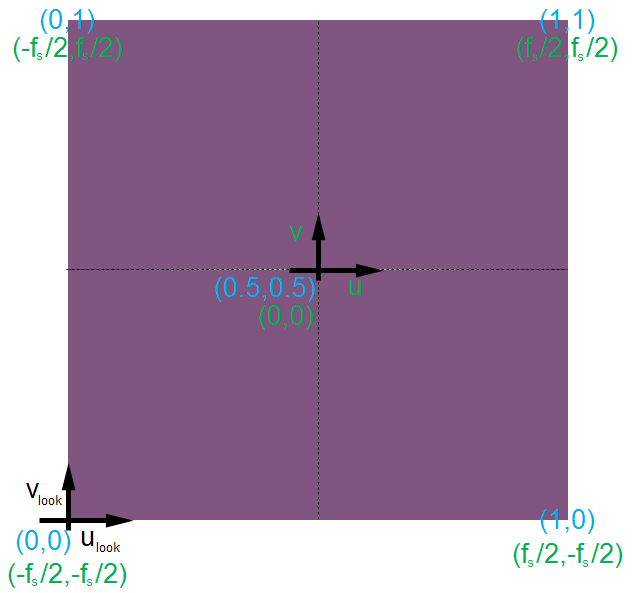
\includegraphics[scale=0.7]{implementation/lookup.png}
  \caption[Lookup DFT Coefficients in Textures]{Illustration of $(u,v)$ lookup using GLSL textures: texture coordinates are shown in blue color, u-v coordinates are shown in green color.}
\label{fig:lookupexample}
\end{figure}

Figure $\ref{fig:lookupexample}$ visualizes a particular DFT coefficients image for a blazed grating. In GLSL texture coordinates the range of such an image is $[0,1]^2$ whereas in a (u,v) coordinates system this would correspond to the range $[-\frac{f_s}{2}, \frac{f_s}{2}]^2$. Regarding the way the DFT terms were computed in Matlab, their zero frequency, i.e. $(u,v) = (0,0)$, is located at the center of the given DFT image. Since by convention the bottom left corner of a GLSL texture corresponds to the origin $(0,0)$ but we want to work with $(u,v)$ coordinates, we have to introduce a helper coordinate system $(u_{lookup}, v_{lookup})$. This helper coordinates can be computed by an affine transformation applied on $(u,v)$ coordinates. Hence, we will explain how to compute the scaling $s$ and translation $b$ components of our affine transformation: 

\myparagraph{Translation component $b$ of affine transformation:}
Since the zero frequency component of DFT images is shifted to its centre position, we have to shift the coordinates $u$ and $v$ to the center of the current $N \times N$ pixel image by a bias $b$ (representing a translation). The translation $b$ is a constant value and is computed like the following:

\begin{align}
b = \left\{ \begin{array}{rl}
\frac{N}{2} &\mbox{ if $N \equiv_2 0$} \\
\frac{N-1}{2} &\mbox{ otherwise}
\end{array} \right.
\label{eq:bias}
\end{align}

\myparagraph{Scaling component $s$ of affine transformation:}
For the scaling part of our affine transformation, we have to think a little further: let us consider a $T$ periodic signal in time, i.e. $x(t) = x(t+nT)$ for any integer $n$. After applying the DFT, we have its discrete spectrum $X[n]$ with frequency interval $w0 = 2pi / T$ and temporal interval $dH$. \\

Let $k$ denote the wavenumber which is equal to $\frac{2 \pi}{\lambda}$ for a given wavelength $\lambda$. Then the signal is both, periodic with time period $T$ and discrete with temporal interval $dH$. This implies that its spectrum should be discrete with frequency interval $w_0$ and periodic with frequency period $\Omega = \frac{2 \pi}{dH}$. This gives us an idea how to discretize the spectrum. For any surface patch $P$ which is periodically distributed on its surface, its frequency interval along the x-axis is equal to: 

\begin{align}
  w_0 = \frac{2 \pi}{T} = \frac{2 \pi}{N \cdot dH}
\end{align}

Thus, only wavenumbers that are integer multiples of $w_0$ after a multiplication with $u$ must be considered, i.e. $ku$ is an integer multiple of $w_0$. Hence the lookup for the $u$-direction will look like:

\begin{align}
    s_{look}(u)
    &=\floor{s(u)}
\label{eq:scalelookdisc}
\end{align}

where 

\begin{align}
    s(u)
    &=\frac{ku}{w_0} \nonumber \\
    &= \frac{ku N dH}{2 \pi} \nonumber \\
    &= \frac{u N dH}{\lambda}
\label{eq:scalelook}
\end{align}

The lookup for the $v$-direction is equal to $s_{look}(v)$ defined as in equation $\ref{eq:scalelookdisc}$. Figure $\ref{fig:susvlook}$ illustrates the difference between $\left( s(u), s(v) \right)$ and its discretized lookup coordinates $\left( s_{look}(u), s_{look}(v) \right)$.

\begin{figure}[H]
  \centering
  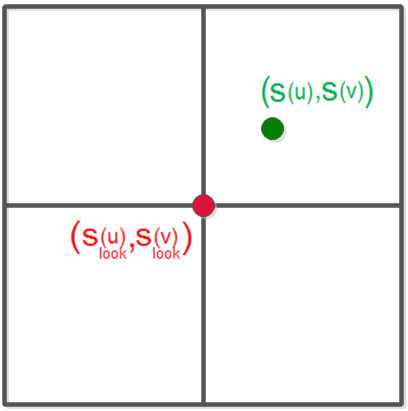
\includegraphics[scale=0.5]{implementation/susvlookidea.png}
  \caption[Discretized Lookup]{Illustration of discrete lookup coordinates $\left( s_{look}(u), s_{look}(v) \right)$.}
\label{fig:susvlook}
\end{figure}


\myparagraph{Final affine transformation:}
Using the translation from equation $\ref{eq:bias}$ and the scaling from equation $\ref{eq:scalelook}$, the transformed texture lookup-coordinates $(u_{look}, v_{look})$ for a given wavelength $\lambda$ is equal to:

\begin{align}
  (u_{look}, v_{look}) 
  &= \left(s_{look}(u)+b,s_{look}(v)+b \right) \nonumber \\
  &= \left( \floor{\frac{u N dH}{\lambda}} + b, \floor{\frac{v N dH}{\lambda}} + b \right)
\label{eq:ublookup}
\end{align}  

Note that for the Windowing Approach, used in algorithm $\ref{alg:fragmentshaderall}$, we are visiting a $n$-pixel-neighborhood around each $(u,v)$ coordinate pair. For any position $(i,j)$ of its neighbor-pixels, these local coordinates $(u_{look}^{local_i}, v_{look}^{local_j})$ around the origin $(u_{look}, v_{look})$ from equation $\ref{eq:ublookup}$ are equal to:

\begin{equation}
  (u_{look}^{local_i}, v_{look}^{local_j}) = (i,j)-(u_{look}, v_{look})
\label{eq:gaussianwindowlook}
\end{equation}

\subsection{Texture Blending}
So far, we have seen how to render structural colors caused by light when diffracted on a grating. But usually, many objects, such as a snake mesh, also have a texture associated with it. Therefore, will have a closer look at how to combine colors of a given texture with computed structural colors. For this purpose we will use a so called texture blending approach. This means that, for each pixel, its final rendered color is a weighted average of different color components, such as the diffraction color, the texture color and the diffuse color. In our shader the diffraction color is weighted by a constant $w_{diffuse}$, denoting the weight of the diffuse color part. The texture color is once scaled by the absolute value of the Fresnel Term $F$ and once by $1-w_{diffuse}$. Algorithm $\ref{alg:textureblending}$ shows in depth how our texture blending is implemented:

\begin{algorithm}[H]
\caption{Texture Blending}
\begin{table}[H]
  \begin{tabular}{@{}lll@{}}
    \textbf{Input:} & $c_{pigmentation}:$ Texture color at given fragment position \\
    & $total_{diffraction}:$ Structural color at given fragment position \\
    \textbf{Output:} & $c_{total}:$ Mixed fragment texture- and structural-color \\
  \end{tabular} 
\end{table}
\setlength{\fboxrule}{0pt} 
\begin{boxedminipage}{1.0\textwidth}
  \begin{algorithmic}[1]

    \State $\alpha = abs(F)$
    \Comment{$\alpha$ is the fraction which goes into the skin}
    \If{$(\alpha > 1)$} \State $\alpha = 1$ \EndIf
    \State $c_{diffraction} = (1-w_{diffuse}) \cdot total_{diffraction}$
    \State $c_{diffuse} = (1-\alpha) \cdot c_{texture}$
    \State $c_{ambient} = w_{diffuse} \cdot c_{pigmentation}$
    \State $c_{total} = c_{diffraction} + c_{diffuse} + c_{ambient}$
  \end{algorithmic}
  \end{boxedminipage}
  \vskip1.5pt
\label{alg:textureblending}
\end{algorithm}

\subsection{Color Transformation}
\label{subsec:colortransformations}

In our fragment shader, we access a table which contains precomputed CIE's color matching functions values$\footnote{Such a function value table can be found at \texttt{cvrl.ioo.ucl.ac.uk} for example}$ from $\lambda_{min} = 380 nm$ to $\lambda_{max} = 780 nm$ in $5 nm$ steps. In algorithm $\ref{alg:fragmentshaderall}$ we describe how to compute the $CIE_{XYZ}$ color values as described in section $\ref{sec:colorspace}$. We can transform the color values into a $CIE_{sRGB}$ gamut by performing the following linear transformation:

\begin{equation}
  \begin{bmatrix}R\\G\\B\end{bmatrix} = M^{-1} \cdot \begin{bmatrix}X\\Y\\Z\end{bmatrix}
\end{equation} 

where one possible transformation for $M$ is: 

\begin{equation}
  M = \begin{bmatrix} 0.41847 & -0.15866 & -0.082835\\ -0.091169 & 0.25243 & 0.015708\\ 0.00092090 & -0.0025498 & 0.17860 \end{bmatrix}
\end{equation}

We may white-balance our results by using the tristimulus value of the color defining the white point in our images. Defining what tristimulus value white corresponds to, usually depends on the application. For our shaders we use the CIE Standard Illuminant $D65$. $D65$ is intended to represent an average midday sun daylight. Applying the D65 illuminant, the whole colorspace transformation will look like:

\begin{equation}
\begin{bmatrix}R\\G\\B\end{bmatrix} = M^{-1} \cdot \begin{bmatrix}X / D65.x \\ Y / D65.y \\Z / D65.z \end{bmatrix} 
\end{equation}

Each component of the Standard Illuminant acts as a rescaling factor according to the white-point definition of $D65$ for our computed color values. Last, we perform a gamma correction on each pixel's $(R,G,B)$ value. A gamma correction is a non linear transformation which controls the overall brightness of an image$\footnote{For further information on gamma correction, please refer the book \emph{Fundamentals of Computer Graphics}$\cite{fundcg}$.}$.

\section{Discussion}
\label{sec:impldiscus}
\subsection{Comparison: per Fragment-vs. per Vertex-Shading}
In this chapter we have seen how our renderer is implemented. We discussed our fragment shader which is responsible for computing the structural color values resulting from diffracted light. Our fragment shader's runtime performance depends on the resolution of the final rendered image, since there is a correspondence between pixels and fragments. Notice that we also could have computed the structural colors during the vertex shading process. Then, the whole rendering performance of our shading approach would only depend on the vertex count of our meshes. Shading on a per vertex basis is usually bad since in order to get a nice and accurate rendering, the vertex count of a mesh has to be big. Furthermore, a vertex shader produces poor results for shapes like a cube for example, according to our structural color model. Therefore, shading on a per fragment shader scales depending on the rendered image resolution and is independent of the mesh vertices (their distribution and count).

\subsection{Optimization of Fragment Shading: NMM Approach}
\label{sec:nmmapproach}
The fragment shader algorithm described in algorithm $\ref{alg:fragmentshaderall}$ performs a gaussian window approach by sampling over the whole wavelength spectrum in uniform step sizes. This algorithm is slow, since iterate over the whole lambda spectrum for each pixel. Furthermore, for any pixel, we iterate over its $n$-neighborhood. When we also consider the number of Taylor series approximation steps, we will have a run-time complexity of

\begin{equation}
O(\#spectrtumIter \cdot \#taylorIter \cdot neighborhoodRadius^2)
\end{equation}
 
Our goal is to optimize this runtime behaviour. Instead of sampling over the whole wavelength spectrum, we could integrate over a minimal number of  wavelengths contributing the most to our shading result like shown in figure $\ref{fig:nmmshadingapproach}$. These values are elicited like the following: Lets consider $(u,v,w)$ defined as in equation $\ref{eq:uvw}$. Let $dH$ denote the resolution for a given discrete height field as described in algorithm $\ref{alg:matlabprecomp}$. For any $L(\lambda) \neq 0$ it follows $\lambda_{n}^{u} = \frac{dH u}{n}$ and $\lambda_{n}^{v} = \frac{dH u}{n}$. Therefore we can derive the following boundaries of $n$:

\label{eq:collectionnmmeqs}
\begin{table}[H]
  \centering 
  \begin{tabular}{l l}
    If $u,v > 0$ & $N_{min}^{u} = \frac{dH u}{\lambda_{max}} \leq n_{u} \leq \frac{dH u}{\lambda_{min}} = N_{min}^{u}$ \\  
    & $N_{min}^{v} = \frac{dH v}{\lambda_{max}} \leq n_{v} \leq \frac{dH v}{\lambda_{min}} = N_{min}^{v}$ \\
    & \\
    If $u,v < 0$ & $N_{min}^{u} = \frac{dH u}{\lambda_{min}} \leq n_{u} \leq \frac{dH u}{\lambda_{min}} = N_{max}^{u}$ \\
    & $N_{min}^{v} = \frac{dH v}{\lambda_{min}} \leq n_{v} \leq \frac{dH v}{\lambda_{min}} = N_{max}^{v}$ \\
    & \\
    If $(u,v)=(0,0)$ & $n_u = 0$ \\
    & $n_v = 0$ \\  
  \end{tabular} 
\end{table}

By transforming those equations (equations $\ref{eq:collectionnmmeqs}$) to $(\lambda_{min}^{u}, \lambda_{min}^{u})$ and $(\lambda_{min}^{v}, \lambda_{min}^{v})$ respectively, we can reduce the total number of required iterations in our fragment shader. We denote this optimization by the $n_{min}$, $n_{max}$ (NMM) shading approach. 

\begin{figure}[H]
  \centering
  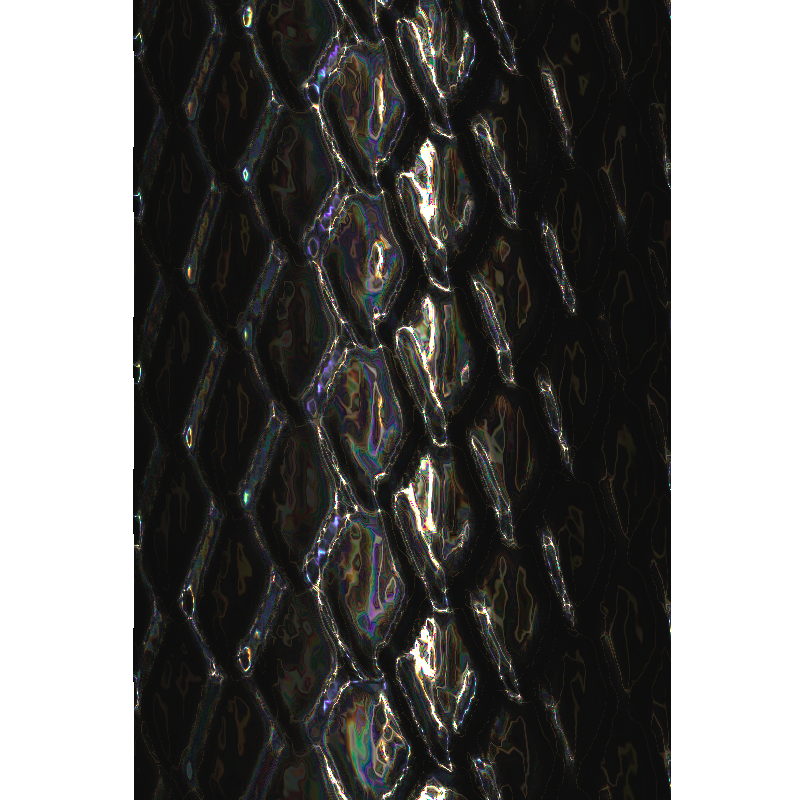
\includegraphics[scale=0.8]{implementation/nmm.png}
  \caption[NMM Shading Approach]{Illustration of NMM shading approach's idea.}
  \label{fig:nmmshadingapproach}
\end{figure}

Figure $\ref{fig:nmmshadingapproach}$ illustrated the idea of the $NMM$ shading approach by showing a visualization of a DFT term. Instead of integrating over the whole wavelength spectrum (yellow line), we can find two constrained wavelength ranges by using equation $\ref{eq:collectionnmmeqs}$. One range is determined by the pair $(N_{min}^{u}, N_{max}^{u})$ (in purple color) and the other by $(N_{min}^{v}, N_{max}^{v})$(in red color). Hence, we only have to integrate once over the reduced, discretized set of $\lambda$ values according to $(N_{min}^{u}, N_{max}^{u})$(red dotted line) and once over $\lambda$ values according to $(N_{min}^{v}, N_{max}^{v})$ (purple dotted line) and then accumulate both results. Since we are uniformly integrating over the wavelength spectrum but this approach selects non-uniformly sampled wavelength spectrum, this can lead to issues. Close to zero frequency, i.e. $(u,v)$ equal to $(0,0)$, we could have too few or even no samples, using the NMM approach. Thus, our workaround according to this issue is to use a default color close to the zero frequency. Technically, this means that white color is returned around a small $\epsilon$ circumstance.

\subsection{The PQ Shading Approach}
\label{sec:pqapproach}
Another variant is the $PQ$ approach described in section $\ref{sec:pq}$. In section $\ref{sec:sincinterpolation}$ we described how to interpolate the values relying on sinc functions. The algorithm of the PQ fragment shader is similar to the FLSS fragment shader described in algorithm $\ref{alg:fragmentshaderall}$. There are only two modifications of algorithm $\ref{alg:fragmentshaderall}$ required:

\begin{enumerate}
  \item Replace the procedure $gaussianWeightOf$ from line 19 by a procedure called $sincWeightOf$.
  \item Multiply $F_{fft}$ at line 23 by an additional weight called $pq$.
\end{enumerate}

The procedure $sincWeightOf$ evaluates the sinc function from equation $\ref{eq:sincinterpolformula}$ and takes as input argument the distance $dist$ defined at line 16 in the algorithm $\ref{alg:fragmentshaderall}$$\footnote{Technically, we multiply this distance by $\pi$, which gives us the an angle used for the sinc function interpolation. Notice that, in order to avoid division by zeros side-effects, we add a small integer $\epsilon$ to our angle value.}$. The $pq$ weight is equal to 

\begin{equation}
  pq = (p^2 + q^2)^{\frac{1}{2}}
\end{equation}

where the factors $p$ and $q$ are defined as in equation $\ref{eq:pqsubst2}$.
